%%%%%%%%%%%%%%%%%%%%%%%%%%%%%%%%%%%%%%%%%%%%%%%%%%%%%%%%%%%%%%%%%%%%
%% I, the copyright holder of this work, release this work into the
%% public domain. This applies worldwide. In some countries this may
%% not be legally possible; if so: I grant anyone the right to use
%% this work for any purpose, without any conditions, unless such
%% conditions are required by law.
%%%%%%%%%%%%%%%%%%%%%%%%%%%%%%%%%%%%%%%%%%%%%%%%%%%%%%%%%%%%%%%%%%%%

\documentclass[
  digital,     %% The `digital` option enables the default options for the
               %% digital version of a document. Replace with `printed`
               %% to enable the default options for the printed version
               %% of a document.
%%  color,       %% Uncomment these lines (by removing the %% at the
%%               %% beginning) to use color in the printed version of your
%%               %% document
  oneside,     %% The `oneside` option enables one-sided typesetting,
               %% which is preferred if you are only going to submit a
               %% digital version of your thesis. Replace with `twoside`
               %% for double-sided typesetting if you are planning to
               %% also print your thesis. For double-sided typesetting,
               %% use at least 120 g/m² paper to prevent show-through.
  nosansbold,  %% The `nosansbold` option prevents the use of the
               %% sans-serif type face for bold text. Replace with
               %% `sansbold` to use sans-serif type face for bold text.
  nocolorbold, %% The `nocolorbold` option disables the usage of the
               %% blue color for bold text, instead using black. Replace
               %% with `colorbold` to use blue for bold text.
  lof,         %% The `lof` option prints the List of Figures. Replace
               %% with `nolof` to hide the List of Figures.
  lot,         %% The `lot` option prints the List of Tables. Replace
               %% with `nolot` to hide the List of Tables.
]{fithesis4}
%% The following section sets up the locales used in the thesis.
\usepackage[resetfonts]{cmap} %% We need to load the T2A font encoding
\usepackage[T1,T2A]{fontenc}  %% to use the Cyrillic fonts with Russian texts.
\usepackage[
  main=english, %% By using `czech` or `slovak` as the main locale
                %% instead of `english`, you can typeset the thesis
                %% in either Czech or Slovak, respectively.
  english, german, russian, czech, slovak %% The additional keys allow
]{babel}        %% foreign texts to be typeset as follows:
%%
%%   \begin{otherlanguage}{german}  ... \end{otherlanguage}
%%   \begin{otherlanguage}{russian} ... \end{otherlanguage}
%%   \begin{otherlanguage}{czech}   ... \end{otherlanguage}
%%   \begin{otherlanguage}{slovak}  ... \end{otherlanguage}
%%
%% For non-Latin scripts, it may be necessary to load additional
%% fonts:
\usepackage{paratype}
\def\textrussian#1{{\usefont{T2A}{PTSerif-TLF}{m}{rm}#1}}
%%
%% The following section sets up the metadata of the thesis.
\thesissetup{
    date        = \the\year/\the\month/\the\day,
    university  = mu,
    faculty     = fi,
    type        = mgr,
    department  = Department of Computer Systems and Communications,
    author      = Bc. Martin Bartoš,
    gender      = m,
    advisor     = {prof. RNDr. Václav Matyáš, M.Sc., Ph.D.},
    title       = {Adaptive Authentication in Keycloak},
    TeXtitle    = {Adaptive Authentication in Keycloak},
    keywords    = {Keycloak, authentication, security, open-source, risk-based, adaptive, Red Hat},
    TeXkeywords = {Keycloak, authentication, security, open-source, risk-based, adaptive, Red Hat},
    abstract    = {%
      Keycloak is an open-source identity and access management system that provides robust security solutions for applications and services. It acts as a centralized authentication and authorization platform, enabling organizations to secure their resources while offering Single Sign-On (SSO) capabilities. Keycloak is widely used in various industries, including web applications, microservices, and APIs, to protect sensitive data and streamline user access control. 
      
      The thesis aims to enhance the security of authentication processes in Keycloak. Traditional static authentication mechanisms, such as username and password, are vulnerable to various security threats, including password breaches, phishing attacks, and unauthorized access. Adaptive authentication might help mitigate these issues. 
      
      Adaptive authentication aims to improve the security posture by dynamically adjusting the authentication requirements based on contextual factors. That means the system can adapt its authentication methods and policies in response to changing circumstances.
    },
    thanks      = {%
      I am deeply grateful to my supervisor, Václav Matyáš, for his guidance and support throughout this thesis. I would also like to thank Marek Posolda for his valuable insights, which greatly enriched this work. Their contributions have been instrumental in its completion.
    },
    bib         = example.bib,
    %% Remove the following line to use the JVS 2018 faculty logo.
    facultyLogo = fithesis-fi,
}
\usepackage{makeidx}      %% The `makeidx` package contains
\makeindex                %% helper commands for index typesetting.
%% These additional packages are used within the document:
\usepackage{paralist} %% Compact list environments
\usepackage{amsmath}  %% Mathematics
\usepackage{amsthm}
\usepackage{amsfonts}
\usepackage{url}      %% Hyperlinks
\usepackage{markdown} %% Lightweight markup
\usepackage{listings} %% Source code highlighting
\usepackage{graphicx}
\lstset{
  basicstyle      = \ttfamily,
  identifierstyle = \color{black},
  keywordstyle    = \color{blue},
  keywordstyle    = {[2]\color{cyan}},
  keywordstyle    = {[3]\color{olive}},
  stringstyle     = \color{teal},
  commentstyle    = \itshape\color{magenta},
  breaklines      = true,
}
\usepackage{floatrow} %% Putting captions above tables
\floatsetup[table]{capposition=top}
\usepackage[babel]{csquotes} %% Context-sensitive quotation marks
\begin{document}
%% The \chapter* command can be used to produce unnumbered chapters:
\chapter*{Introduction}
%% Unlike \chapter, \chapter* does not update the headings and does not
%% enter the chapter to the table of contents. I we want correct
%% headings and a table of contents entry, we must add them manually:
\markright{\textsc{Introduction}}
\addcontentsline{toc}{chapter}{Introduction}

TODO
In today's digital landscape, where cybersecurity threats continue to evolve in sophistication and frequency, the need for robust authentication mechanisms to safeguard sensitive data and systems has become paramount.
Traditional authentication methods, such as static passwords or even static multi-factor authentication (MFA), often fall short of adequately addressing the dynamic nature of security risks and user behavior.
As a response to these challenges, adaptive authentication has emerged as a promising approach to authentication, offering a dynamic and context-aware method for verifying user identities.

This thesis aims to explore the principles, mechanisms, benefits, and challenges of adaptive authentication in-depth.
By examining the underlying concepts and technologies, as well as conducting case studies and analyses, this research seeks to provide insights into the effectiveness and applicability of adaptive authentication solutions in diverse organizational contexts.
Through a comprehensive examination of adaptive authentication, this thesis aims to contribute to the understanding of modern authentication practices and their role in mitigating cybersecurity risks.

\shorthandoff{-}
\begin{markdown*}{%
  hybrid,
  definitionLists,
  footnotes,
  inlineFootnotes,
  hashEnumerators,
  fencedCode,
  citations,
  citationNbsps,
  pipeTables,
  tableCaptions,
}
\chapter{Adaptive Authentication}
\section{Introduction}
Adaptive authentication is an advanced security mechanism designed to dynamically adjust the level of authentication required for accessing digital systems, applications, or data based on various factors such as user behavior, context, and risk levels.
Unlike traditional authentication methods that rely on static credentials or fixed multi-factor authentication (MFA) processes, adaptive authentication continuously evaluates the risk associated with each authentication attempt and adapts the authentication requirements accordingly.

At its core, adaptive authentication leverages real-time data analysis and contextual insights to make informed decisions about the appropriate level of authentication needed to verify a user's identity.
This dynamic approach allows organizations to strengthen security measures while minimizing disruption to user workflows.
Unlike static authentication methods, which apply the exact authentication requirements to all users and sessions, adaptive authentication systems continuously evaluate risk factors and adjust authentication measures accordingly.

By leveraging real-time data and analytical capabilities, adaptive authentication enhances security while also optimizing the user experience.
\newpage
\section{Benefits}
As was stated in the introduction of Adaptive Authentication, the main benefits behind its usability are mainly the dynamics.
As in the traditional approaches, the static MFA is very often used when assessing authentication policies with predefined exact rules that the user might comply with or the system's state is in.

Adaptive Authentication provides the ability to have a more frictionless approach when a user is trying to prove their identity.
\newline
\newline
The summarization of the more exciting benefits might be as follows:

% https://www.silverfort.com/glossary/adaptive-authentication/#adaptive-authentication-vs-traditional-authentication-pros-and-cons
% https://www.descope.com/learn/post/adaptive-authentication#benefits-and-drawbacks-of-adaptive-authentication
% https://www.logintc.com/types-of-authentication/adaptive-authentication/
% https://www.incognia.com/the-authentication-reference/what-is-adaptive-authentication

\begin{itemize}
    \item \textbf{Better user experience} - provides more frictionless authentication as a user is not required to provide too many aspects of their identity
    \item \textbf{Strengthen security} - when a user is trying to access sensitive or important resources, additional factors might be required
    \item \textbf{Context-Aware protection} - takes into account contextual information, such as device information, location, IP address, and behavioral patterns
    \item \textbf{Flexibility and extendability} - by leveraging more contextual data, the policies and rules might better comply with customers' needs
    \item \textbf{Integration with AI/ML} - Artificial Intelligence, or Machine learning, might be used for processing contextual data, assessing risk levels, and making more knowledgeable decisions
    \item \textbf{Alignment with zero trust model} - Adaptive authentication aligns well with the Zero trust security model due to its main principle to 'never trust, always verify'
\end{itemize}

\newpage
\section{Challenges}
While the benefits of adaptive authentication are clear and compelling, it's essential to acknowledge that this approach might face several challenges.
Despite its dynamic nature and improved user experience, adaptive authentication presents several challenges that organizations must address to realize its full potential.
\newline
\newline
The summarization of the biggest challenges might be as follows:

% https://www.silverfort.com/glossary/adaptive-authentication/#adaptive-authentication-vs-traditional-authentication-pros-and-cons
% https://www.descope.com/learn/post/adaptive-authentication#benefits-and-drawbacks-of-adaptive-authentication
% https://www.logintc.com/types-of-authentication/adaptive-authentication/

\begin{itemize}
    \item \textbf{Complexity} - the implementation of the processing user behavior and evaluation of contextual data might be very complex and time-consuming  
    \item \textbf{Accuracy of Risk Assessment} - as the contextual data might not be reliable and correct in a particular context, the risk evaluation needs to be properly executed - we need to prevent count of false positives and false negatives 
    \item \textbf{Privacy and Data protection} - as the contextual data might help to strengthen security, these data need to be collected and processed - compliance with data protection regulations and users' preferences needs to be assessed.
    \item \textbf{Potentially non-deterministic} - the benefit of integration of AI/ML might also bring some challenges as we can achieve non-deterministic behavior in processing contextual data and assessing risk levels - it might be challenging to predict possible outcomes, which also makes testing harder
    
\end{itemize}

\newpage
\section{Authentication factors}
Authentication factors play a crucial role in verifying the identity of users and granting them access to digital systems, applications, and data.
In the realm of cybersecurity, authentication factors serve as the building blocks of authentication mechanisms, providing layers of security to protect against unauthorized access and mitigate the risk of security breaches.

Authentication factors exist to address the inherent limitations and vulnerabilities of traditional password-based authentication methods.
While passwords have long been the primary means of authenticating users, they are susceptible to various security threats, such as brute-force attacks, phishing, and password reuse.
Authentication factors enhance security by introducing additional layers of verification beyond mere knowledge of a password.

% https://www.aratek.co/news/5-authentication-factors-a-guide-from-passwords-to-biometrics
% https://www.descope.com/learn/post/mfa
%https://rublon.com/blog/what-are-the-three-authentication-factors/

Adaptive Authentication uses Authentication factors to evaluate the potential risk that a user accessing a particular resource is fraudulent.
\newline
\newline
These factors use contextual data obtained by arbitrary approaches and can be divided into a few categories:

\begin{enumerate}
    \item \textbf{Knowledge factor} (Something You Know)
    \item \textbf{Possession factor}  (Something You Have)
    \item \textbf{Inherence factor} (Something You Are)
    \item \textbf{Location factor} (Somewhere You Are)
    \item \textbf{Behavior factor} (Something You Do)
\end{enumerate}

The first three authentication factors \textit{Knowledge factor}, \textit{Posession factor}, and \textit{Inherence factor} are the well-known traditional factors used in many applications managing identity access.
The last two authentication factors \textit{Location factor}, and \textit{Behavior factor}, are the extension of the traditional approaches and extensively used for the Adaptive authentication.  

\newpage
\subsection{Knowledge factor (Something You Know)}
Knowledge factors involve users providing specific information or data to access a secured system.
The most common type of knowledge-based authentication is through passwords or personal identification numbers (PINs), which are used to limit system access.

Typically, in generic applications or network logins, users need to provide both a username/email and its associated password or PIN to gain entry. It is important to note that solely providing a username or email does not serve as an authentication factor.
Instead, it functions as the user's identification within the system.

Authentication occurs when the provided password or PIN verifies the associated username or email, confirming the user's identity.

\begin{figure}[htbp]
  \centering
  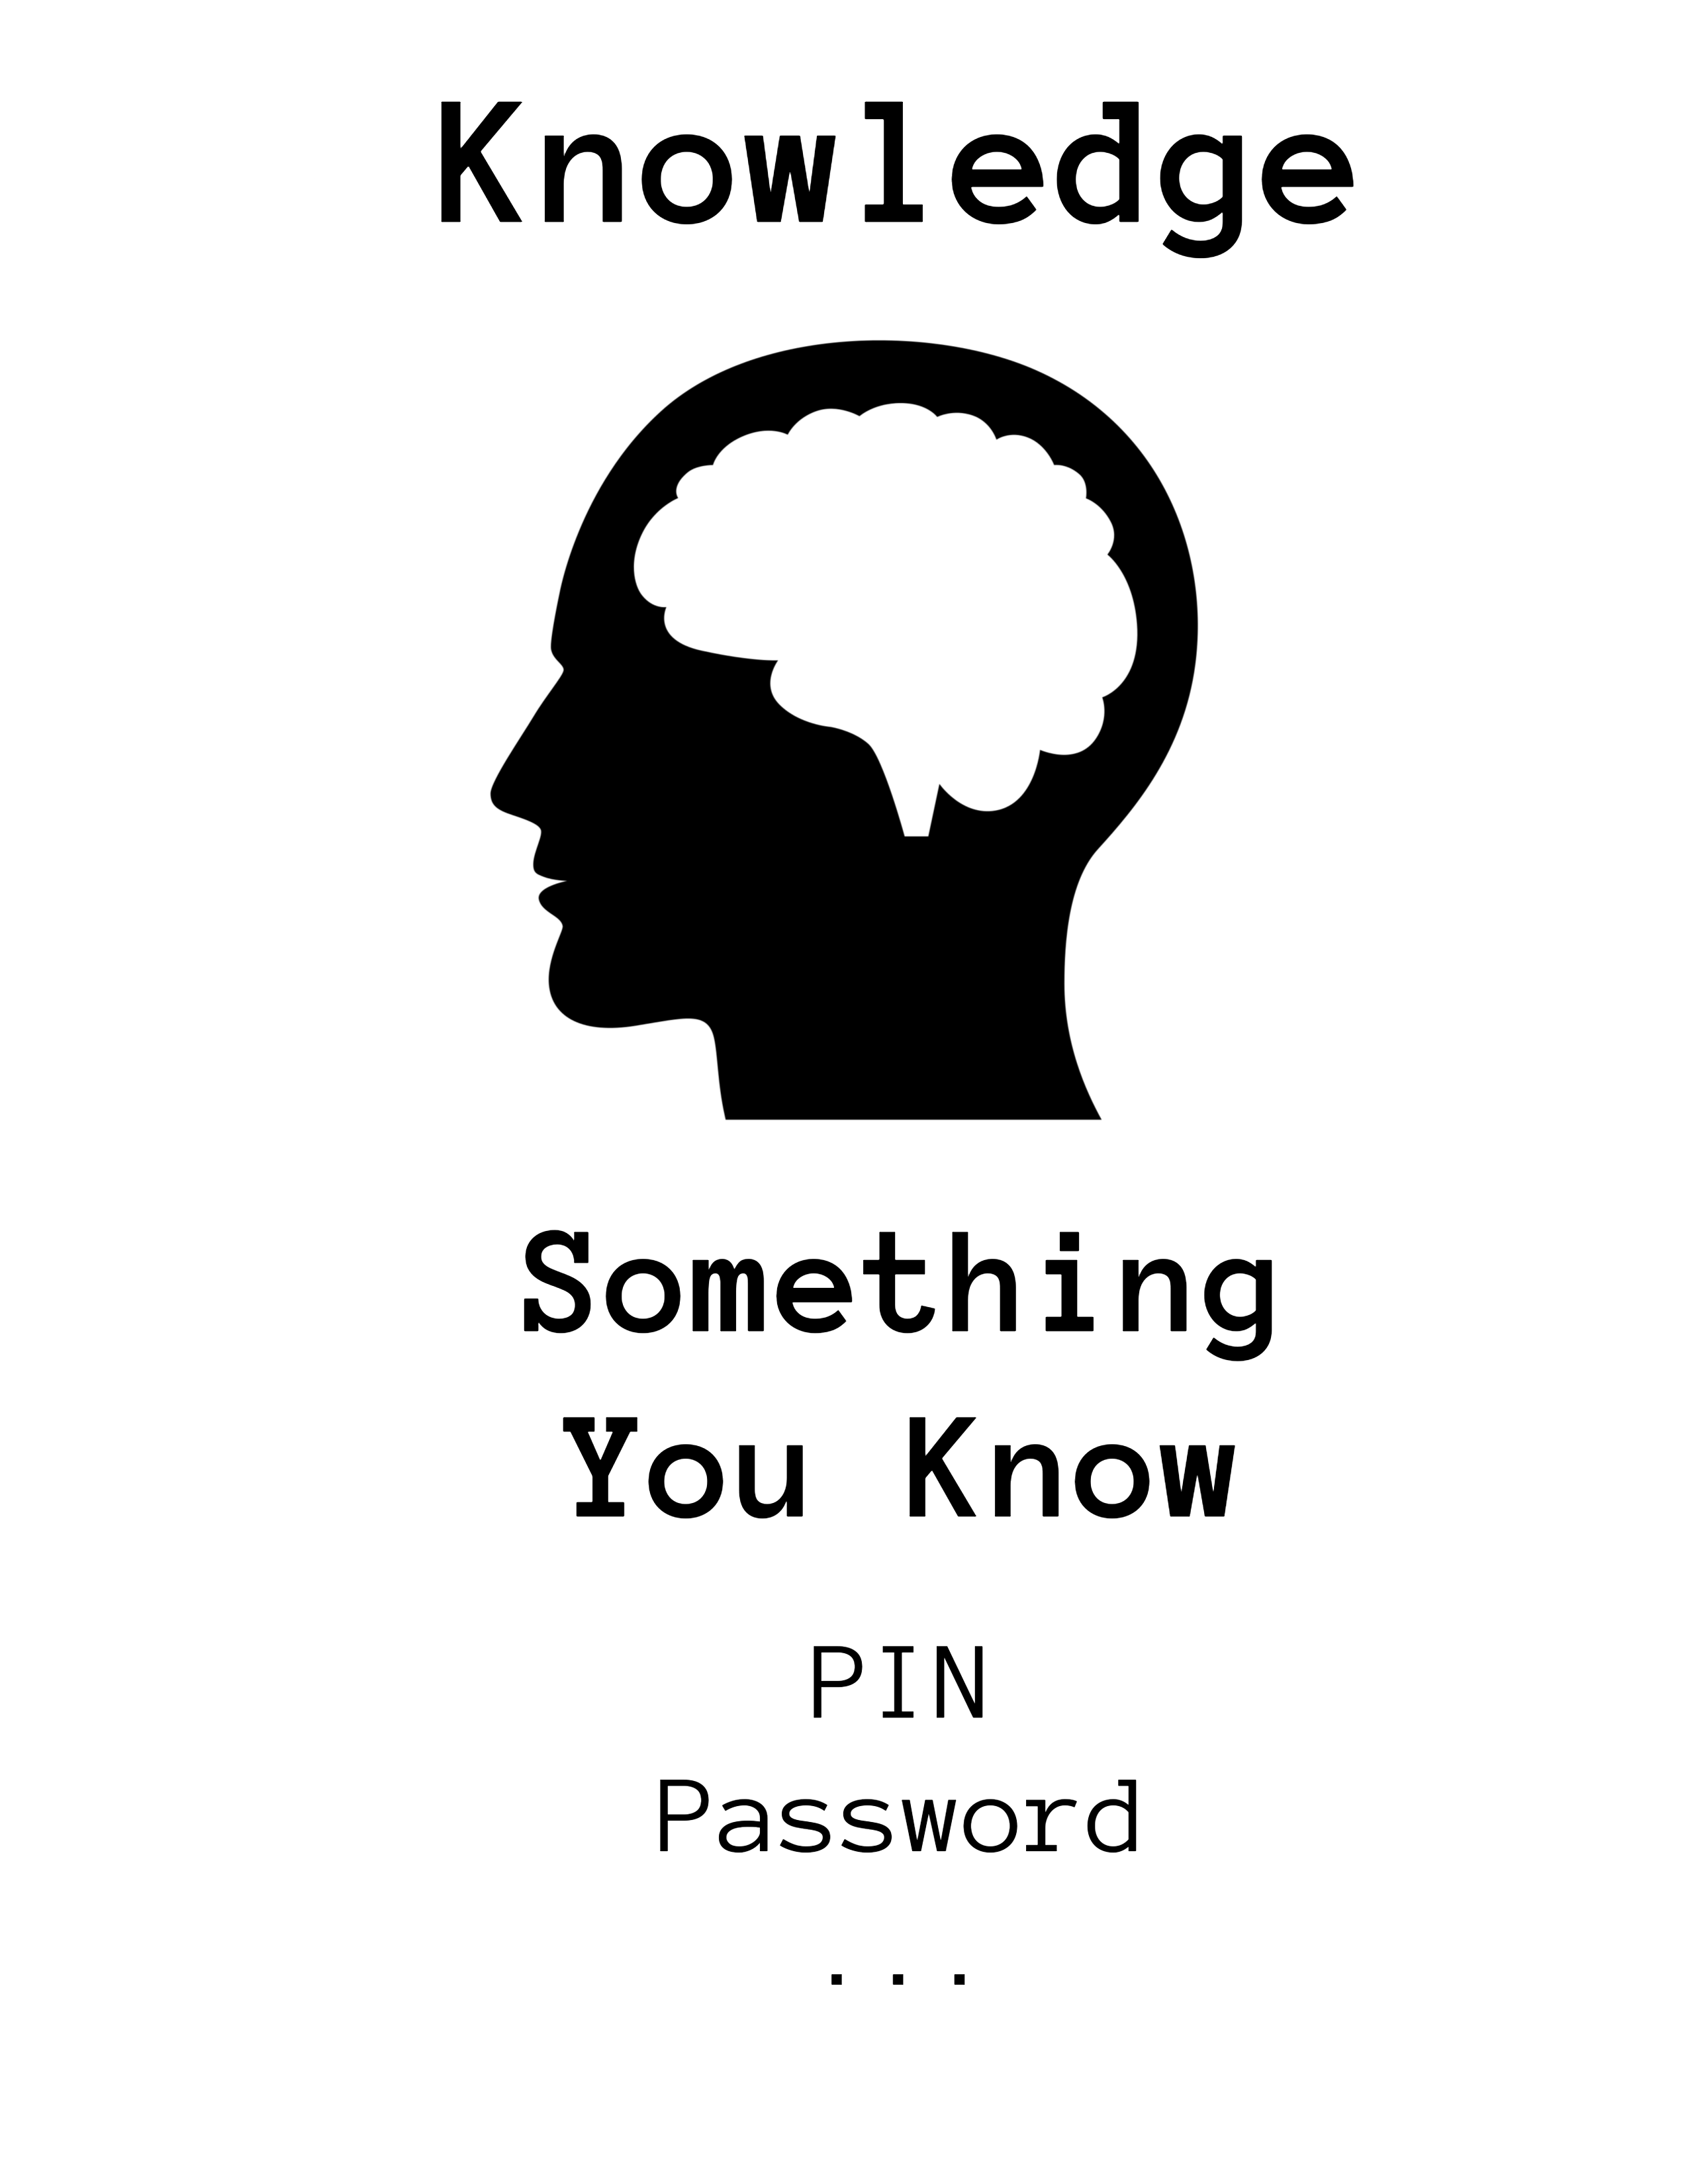
\includegraphics[width=0.6\textwidth]{img/knowledge-final.png}
  \caption{Knowledge factor}
  \label{fig:knowledge-factor}
\end{figure}

\newpage
\subsection{Possession factor (Something You Have)}
Possession factors require users to possess a specific piece of information or device before gaining access to the system.
Typically, possession factors are managed through a device known to belong to the correct user.
A typical process flow for possession-based authentication might look like described in the following lines.

The user registers an account with a password and their phone number recorded at the time of registration.
The user logs in to their account with the username and password.
When the user requests access to the system, a one-time password is generated and sent to the user's mobile phone number.
The user enters the newly generated one-time password and gains access to the system.

One-time passwords can be generated by a device like the RSA SecurID, or they may be automatically generated and sent to the user's cellular device via SMS.
In either case, the correct user must possess the device that receives or generates the one-time password to access the system.

\begin{figure}[htbp]
  \centering
  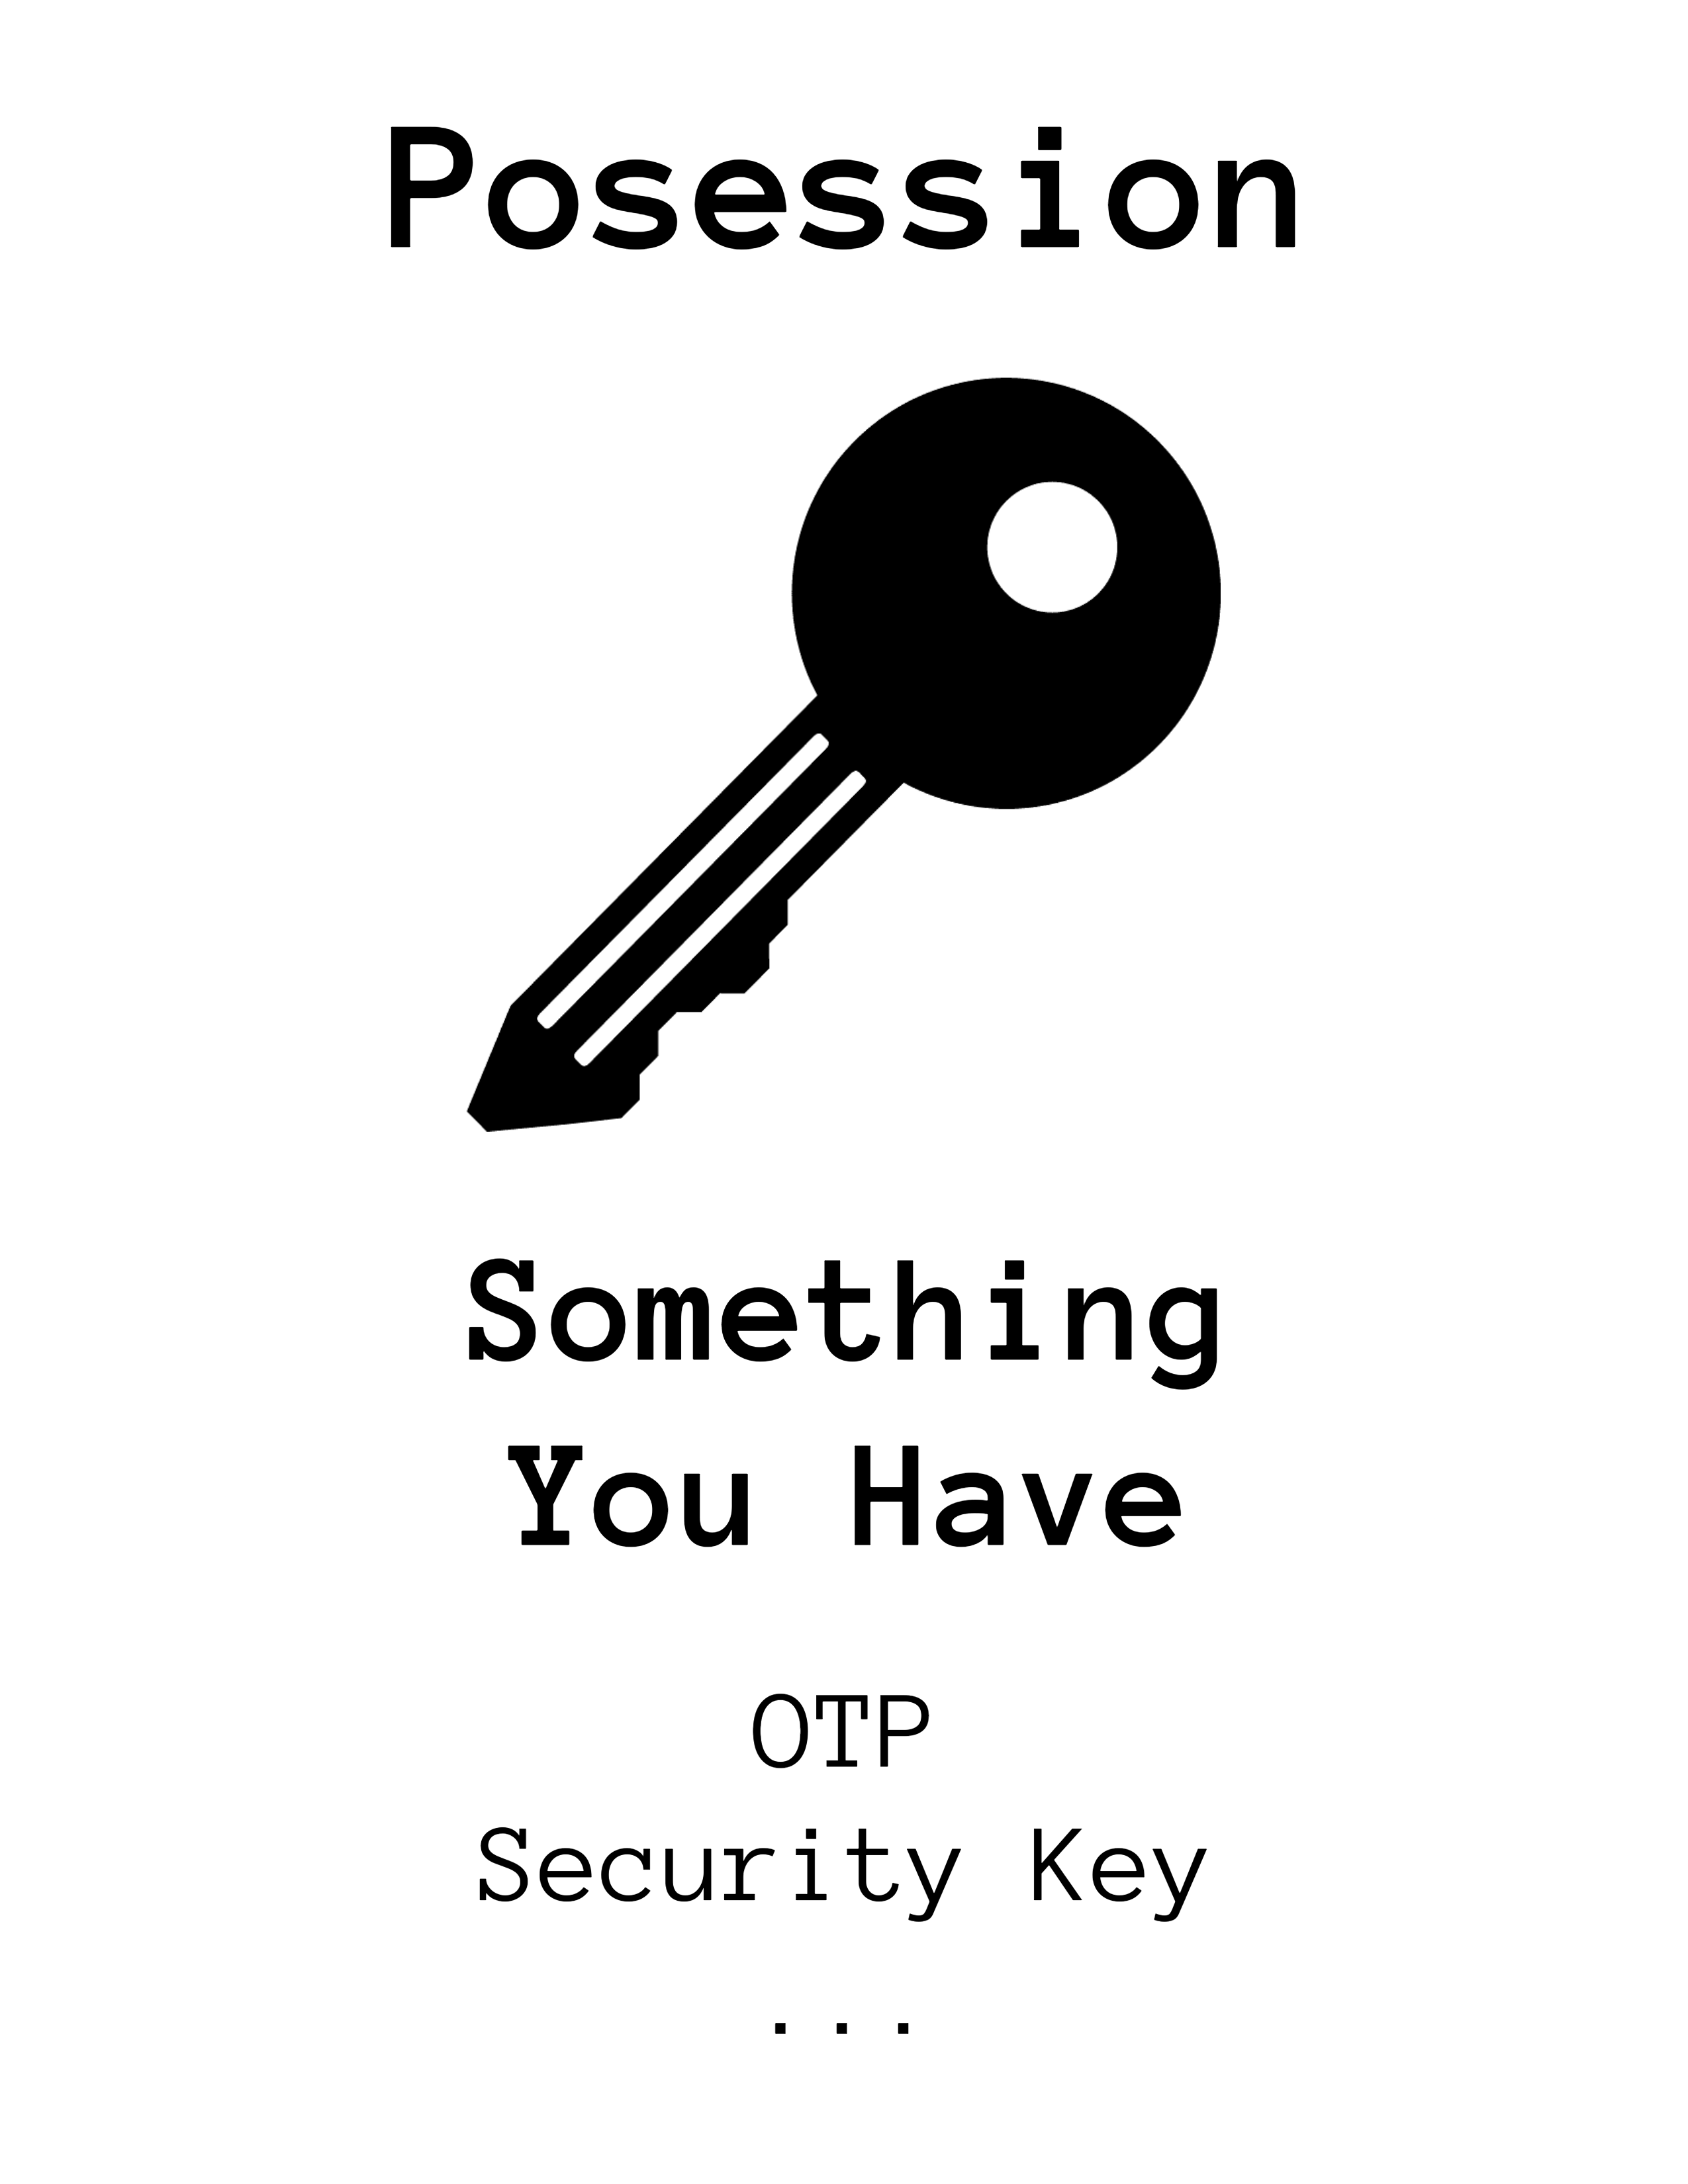
\includegraphics[width=0.53\textwidth]{img/posession-final.png}
  \caption{Posession factor}
  \label{fig:posession-factor}
\end{figure}

\newpage
\subsection{Inherence factor (Something You Are)}
Inherence factors authenticate access credentials based on unique user characteristics.
These include fingerprints, thumbprints, palm or handprints, as well as voice and facial recognition and retina or iris scans.

When systems proficiently identify users via their biometric data, inherence stands as one of the most secure authentication methods.
However, a downside is the potential loss of flexibility in account access.

For instance, a system requiring a fingerprint scan can only be accessed on devices equipped with the necessary hardware.
While this restriction enhances security, it may diminish user convenience.

\begin{figure}[htbp]
  \centering
  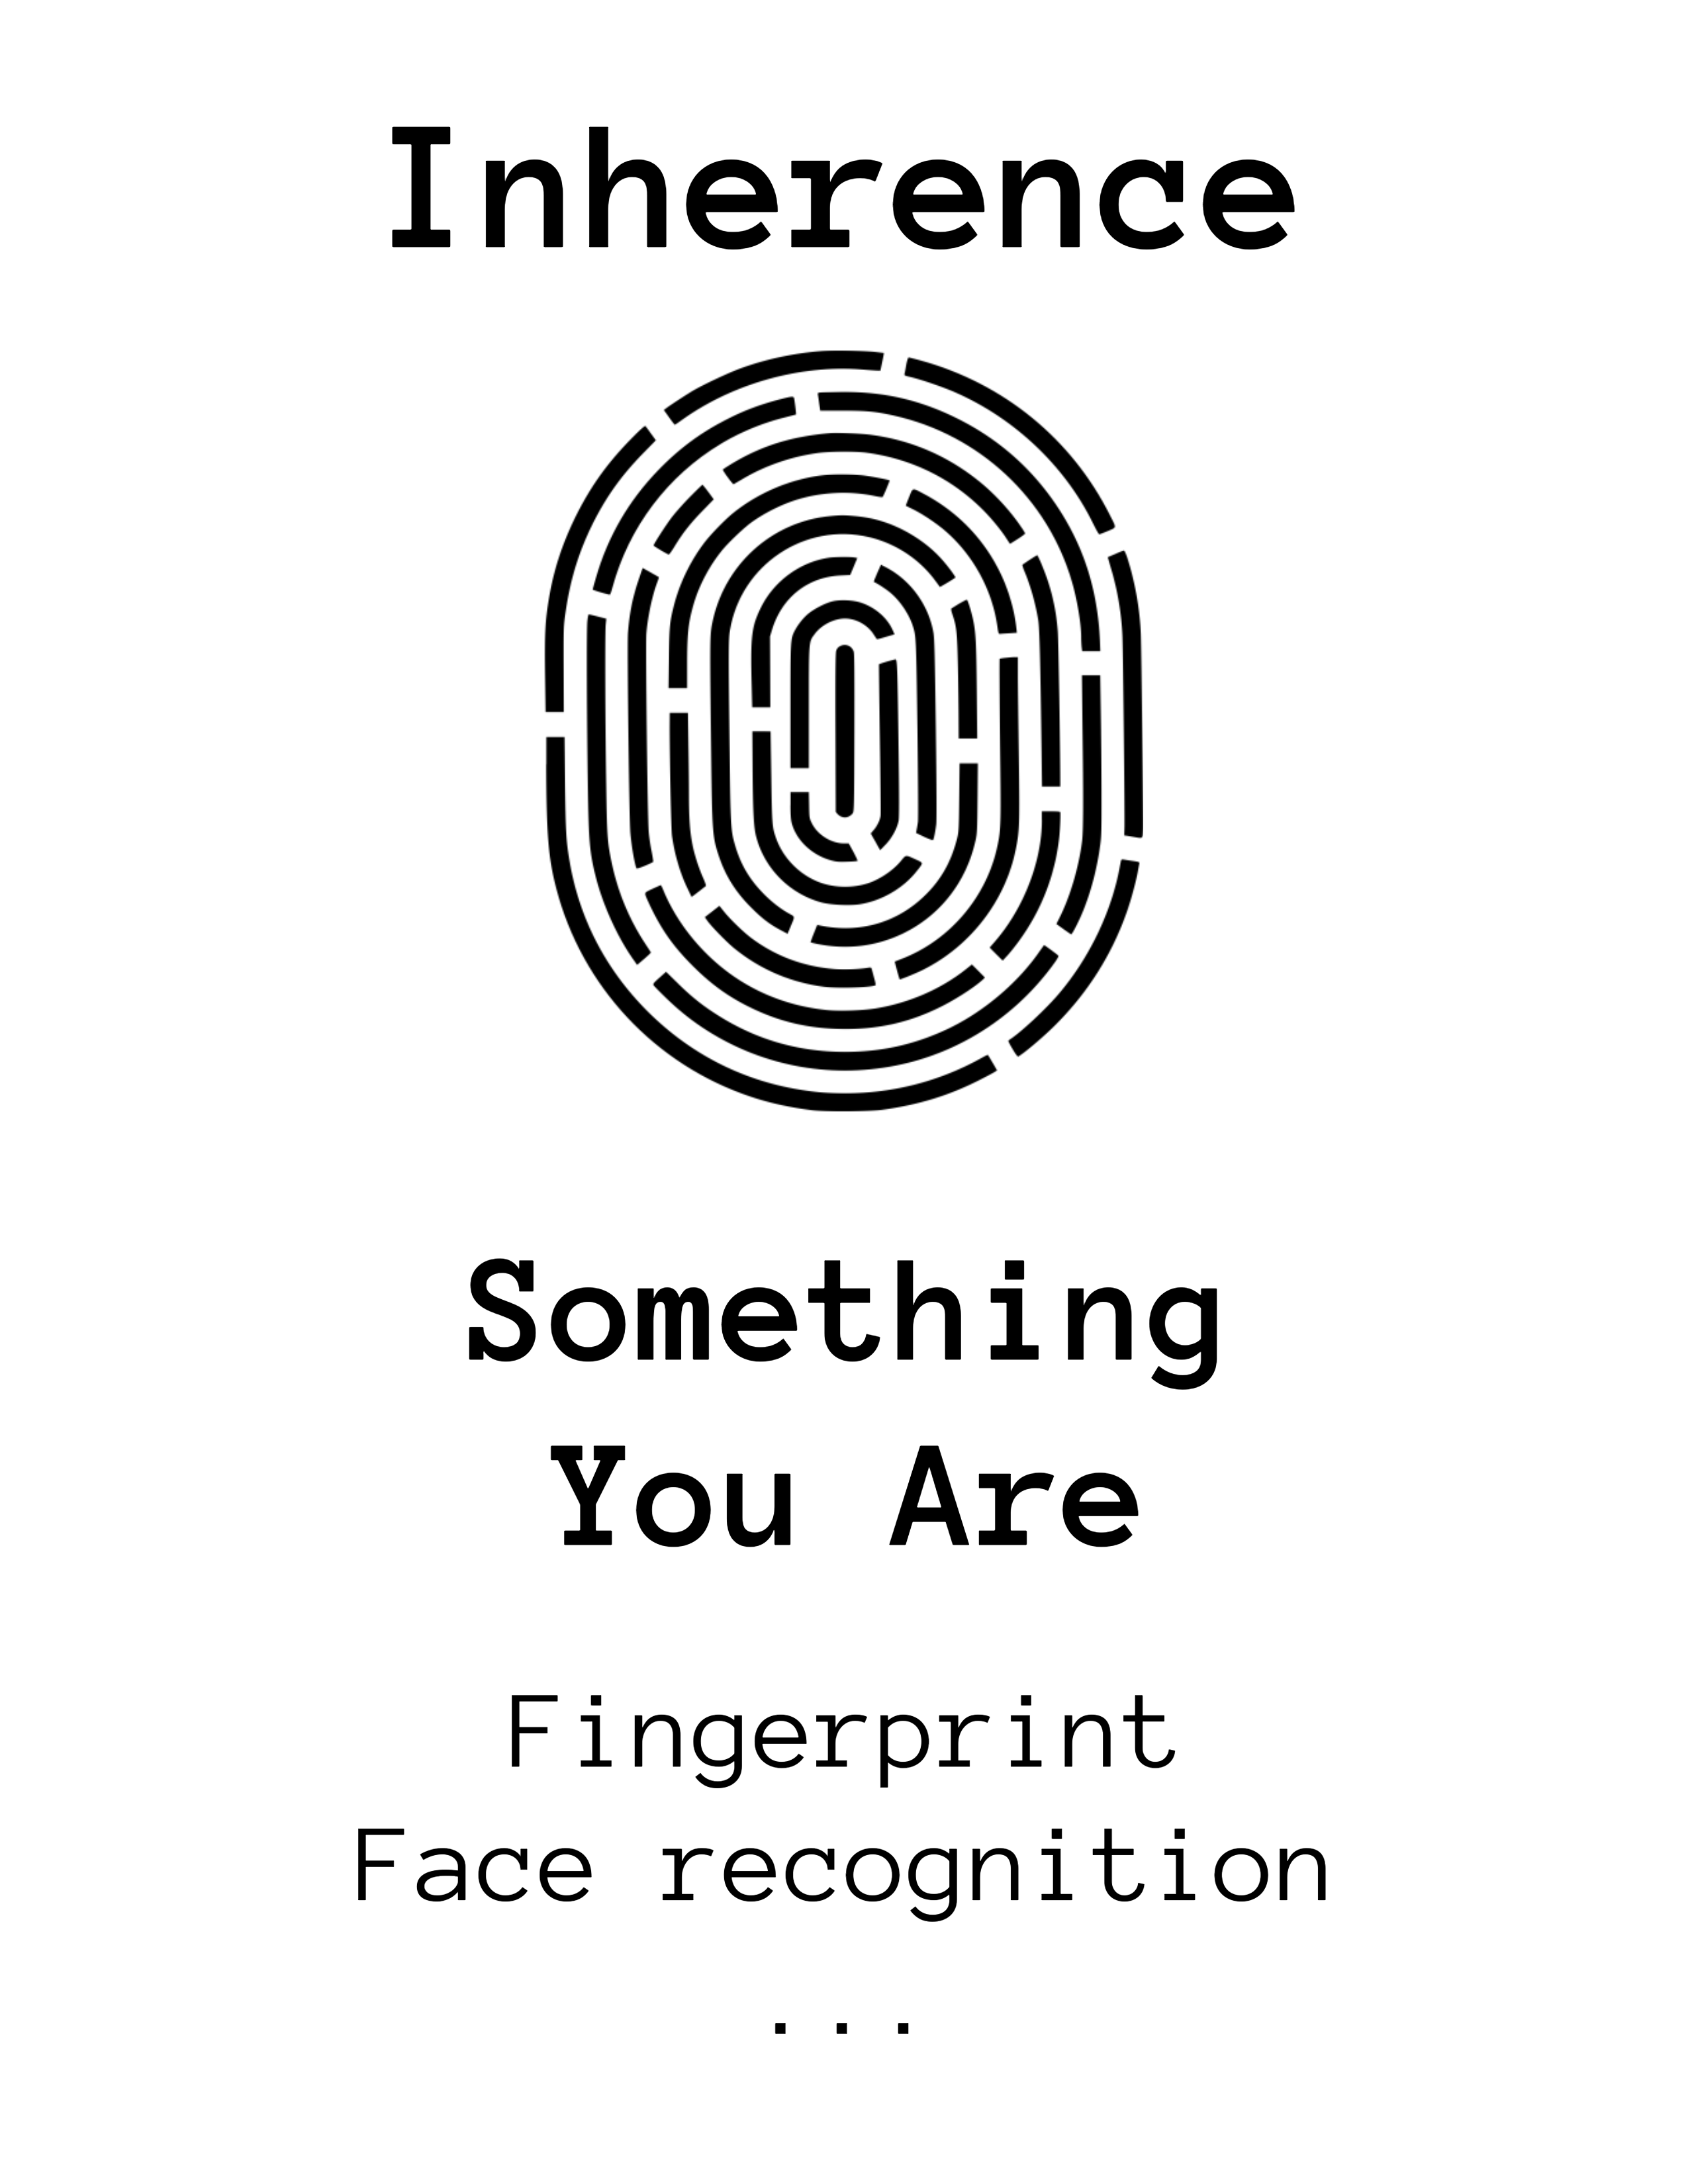
\includegraphics[width=0.55\textwidth]{img/inherence-final.png}
  \caption{Inherence factor}
  \label{fig:inherence-factor}
\end{figure}

\newpage
\subsection{Location factor (Somewhere You Are)}
Location factors allow administrators to implement geolocation security checks to verify a user's location before granting access to an application, network, or system.

Consider a multinational corporation with offices in various cities worldwide.
In this scenario, a security analyst might identify a user attempting to access the network from an IP address originating from a country different from their assigned office as a potential cyber attacker or unauthorized entity.

Geolocation security ensures access is restricted to users within a specified geographic area.
While IP addresses offer insight into network traffic origin, hackers can avoid detection by using VPNs to mask their location.

Alternatively, MAC addresses, unique to each computing device, can serve as a location-based authentication factor, allowing system access only from authorized devices within a defined range.

\begin{figure}[htbp]
  \centering
  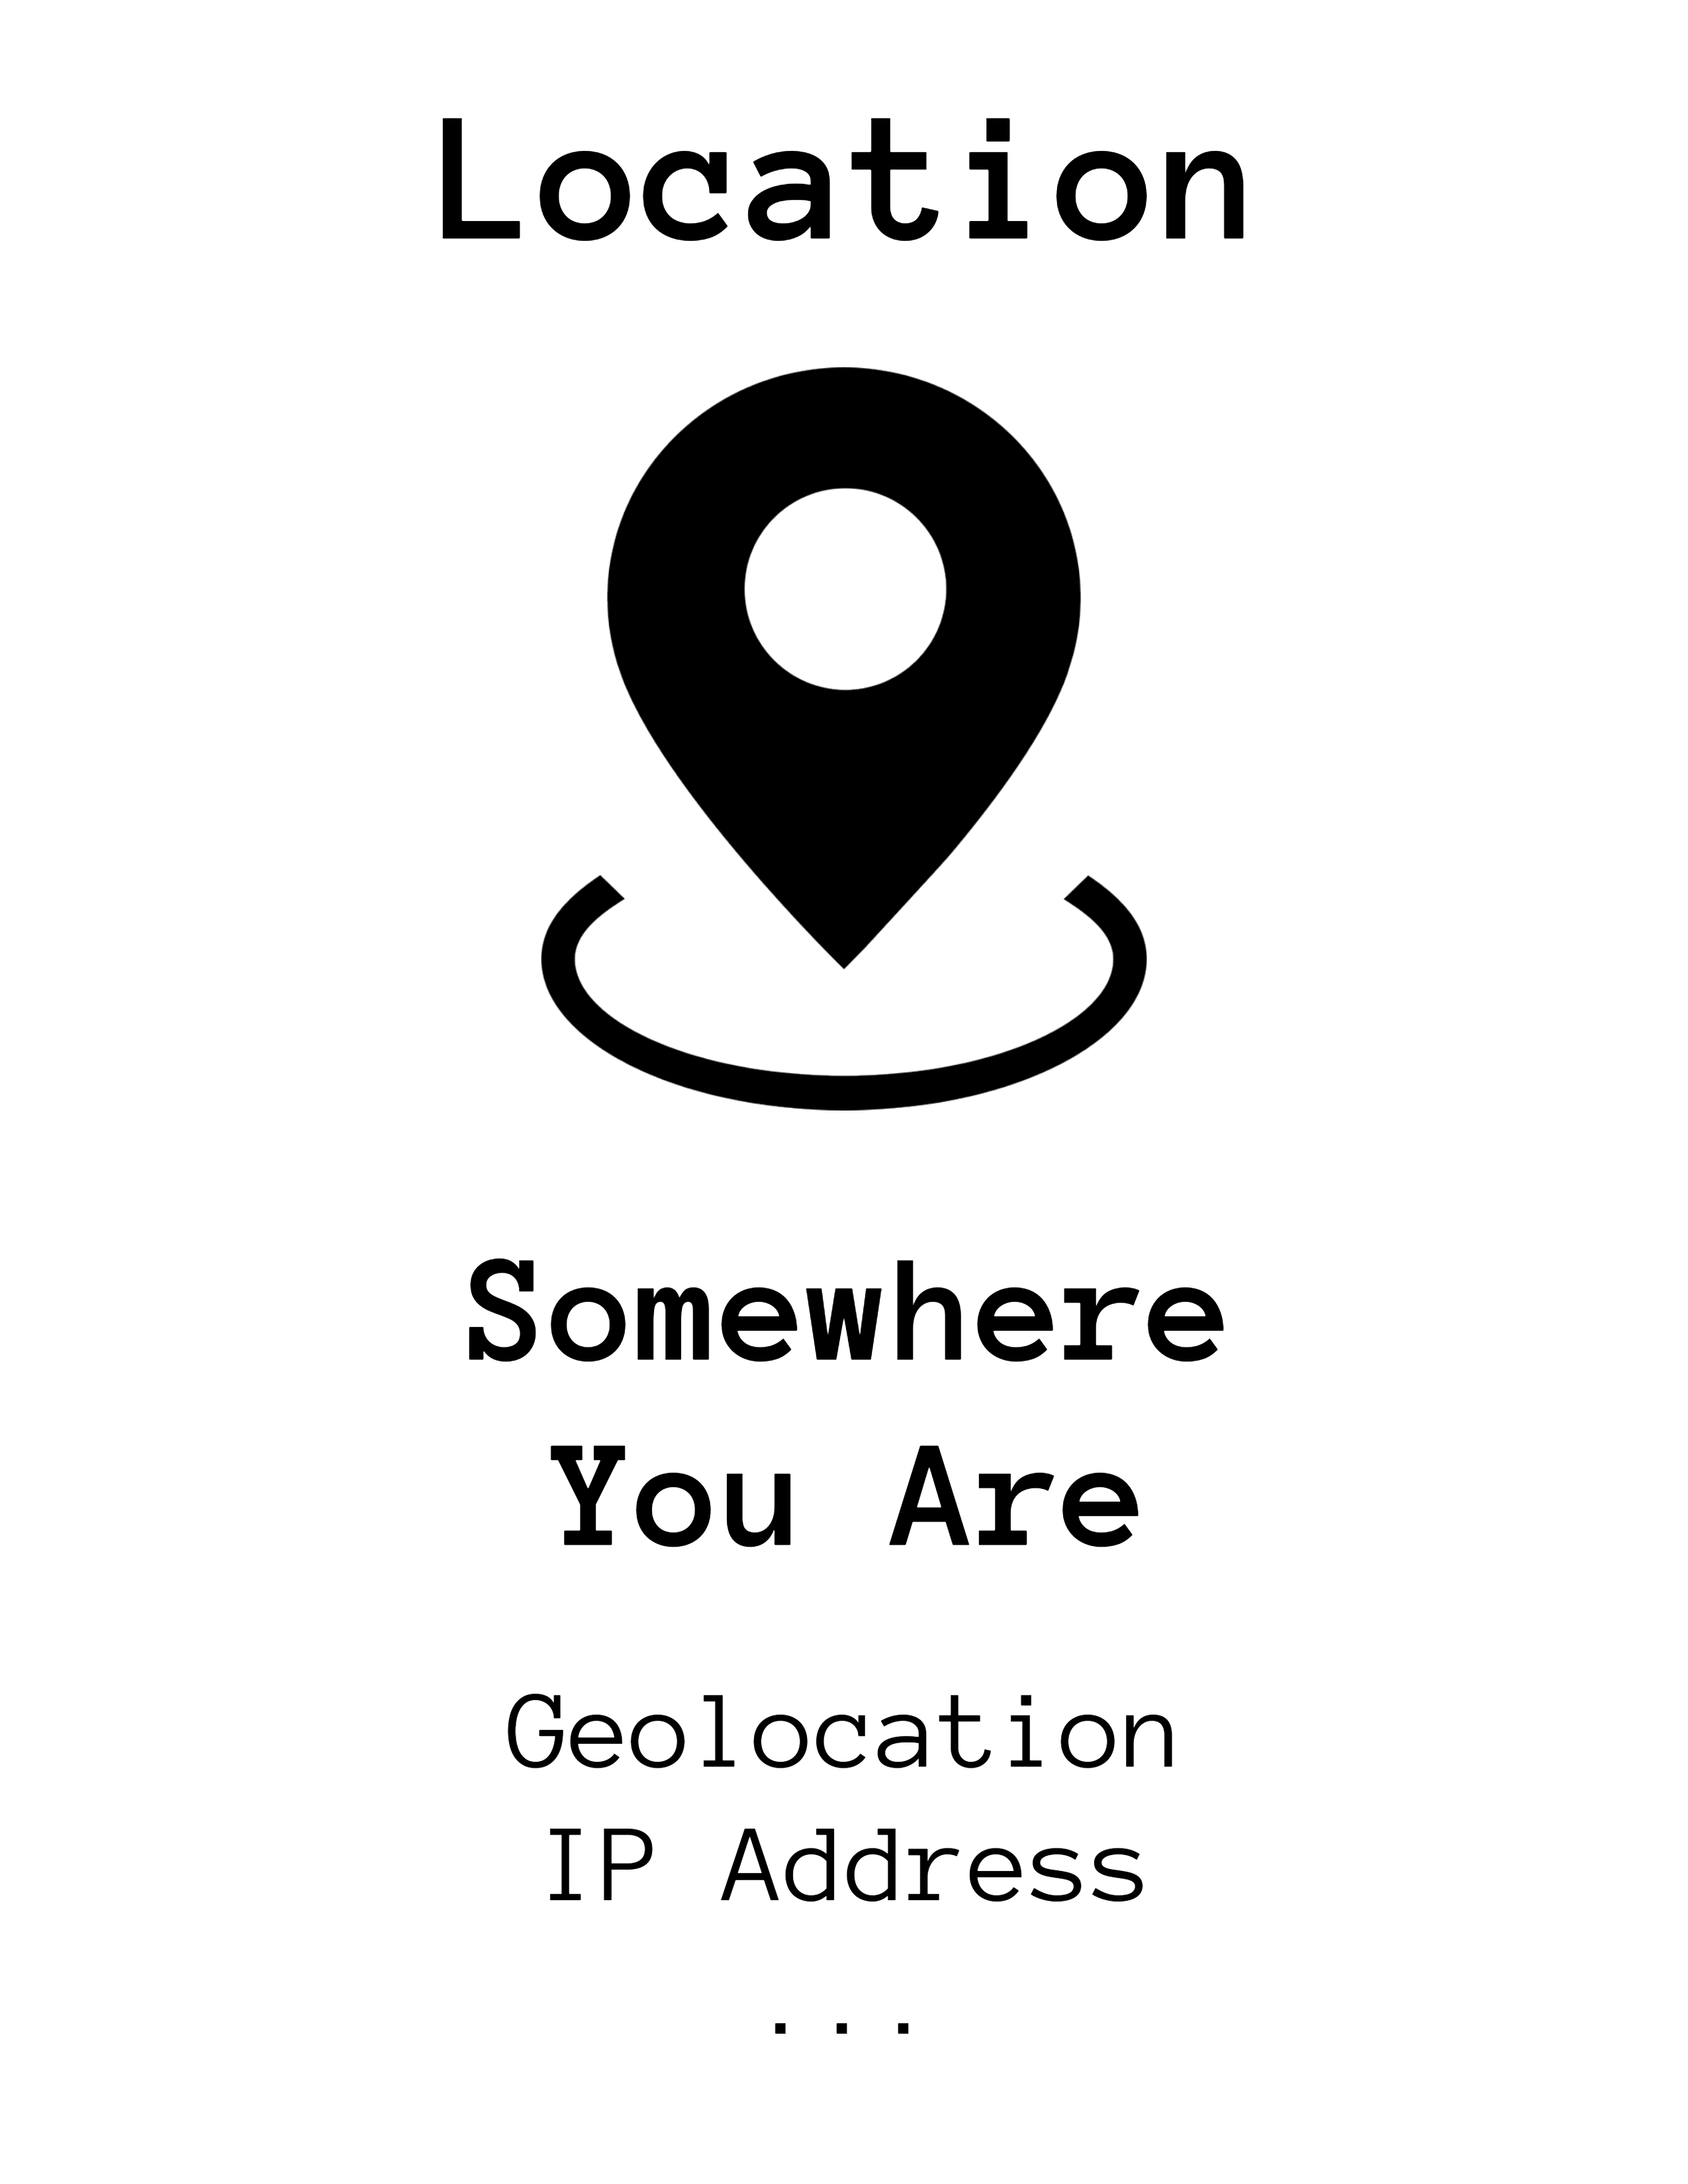
\includegraphics[width=0.55\textwidth]{img/location-final.png}
  \caption{Location factor}
  \label{fig:location-factor}
\end{figure}

\newpage
\subsection{Behavior factor (Something You Do)}
Behavior factors depend on user actions to access the system. In systems accommodating behavior-based authentication factors, users may configure a password by executing specific actions within a defined interface, which they can subsequently replicate to verify their identity.

Consider the gesture-based authentication feature found in some smartwatches, where users perform a series of taps or swipes to unlock the device. This serves as an example of behavior-based authentication factors.

\begin{figure}[htbp]
  \centering
  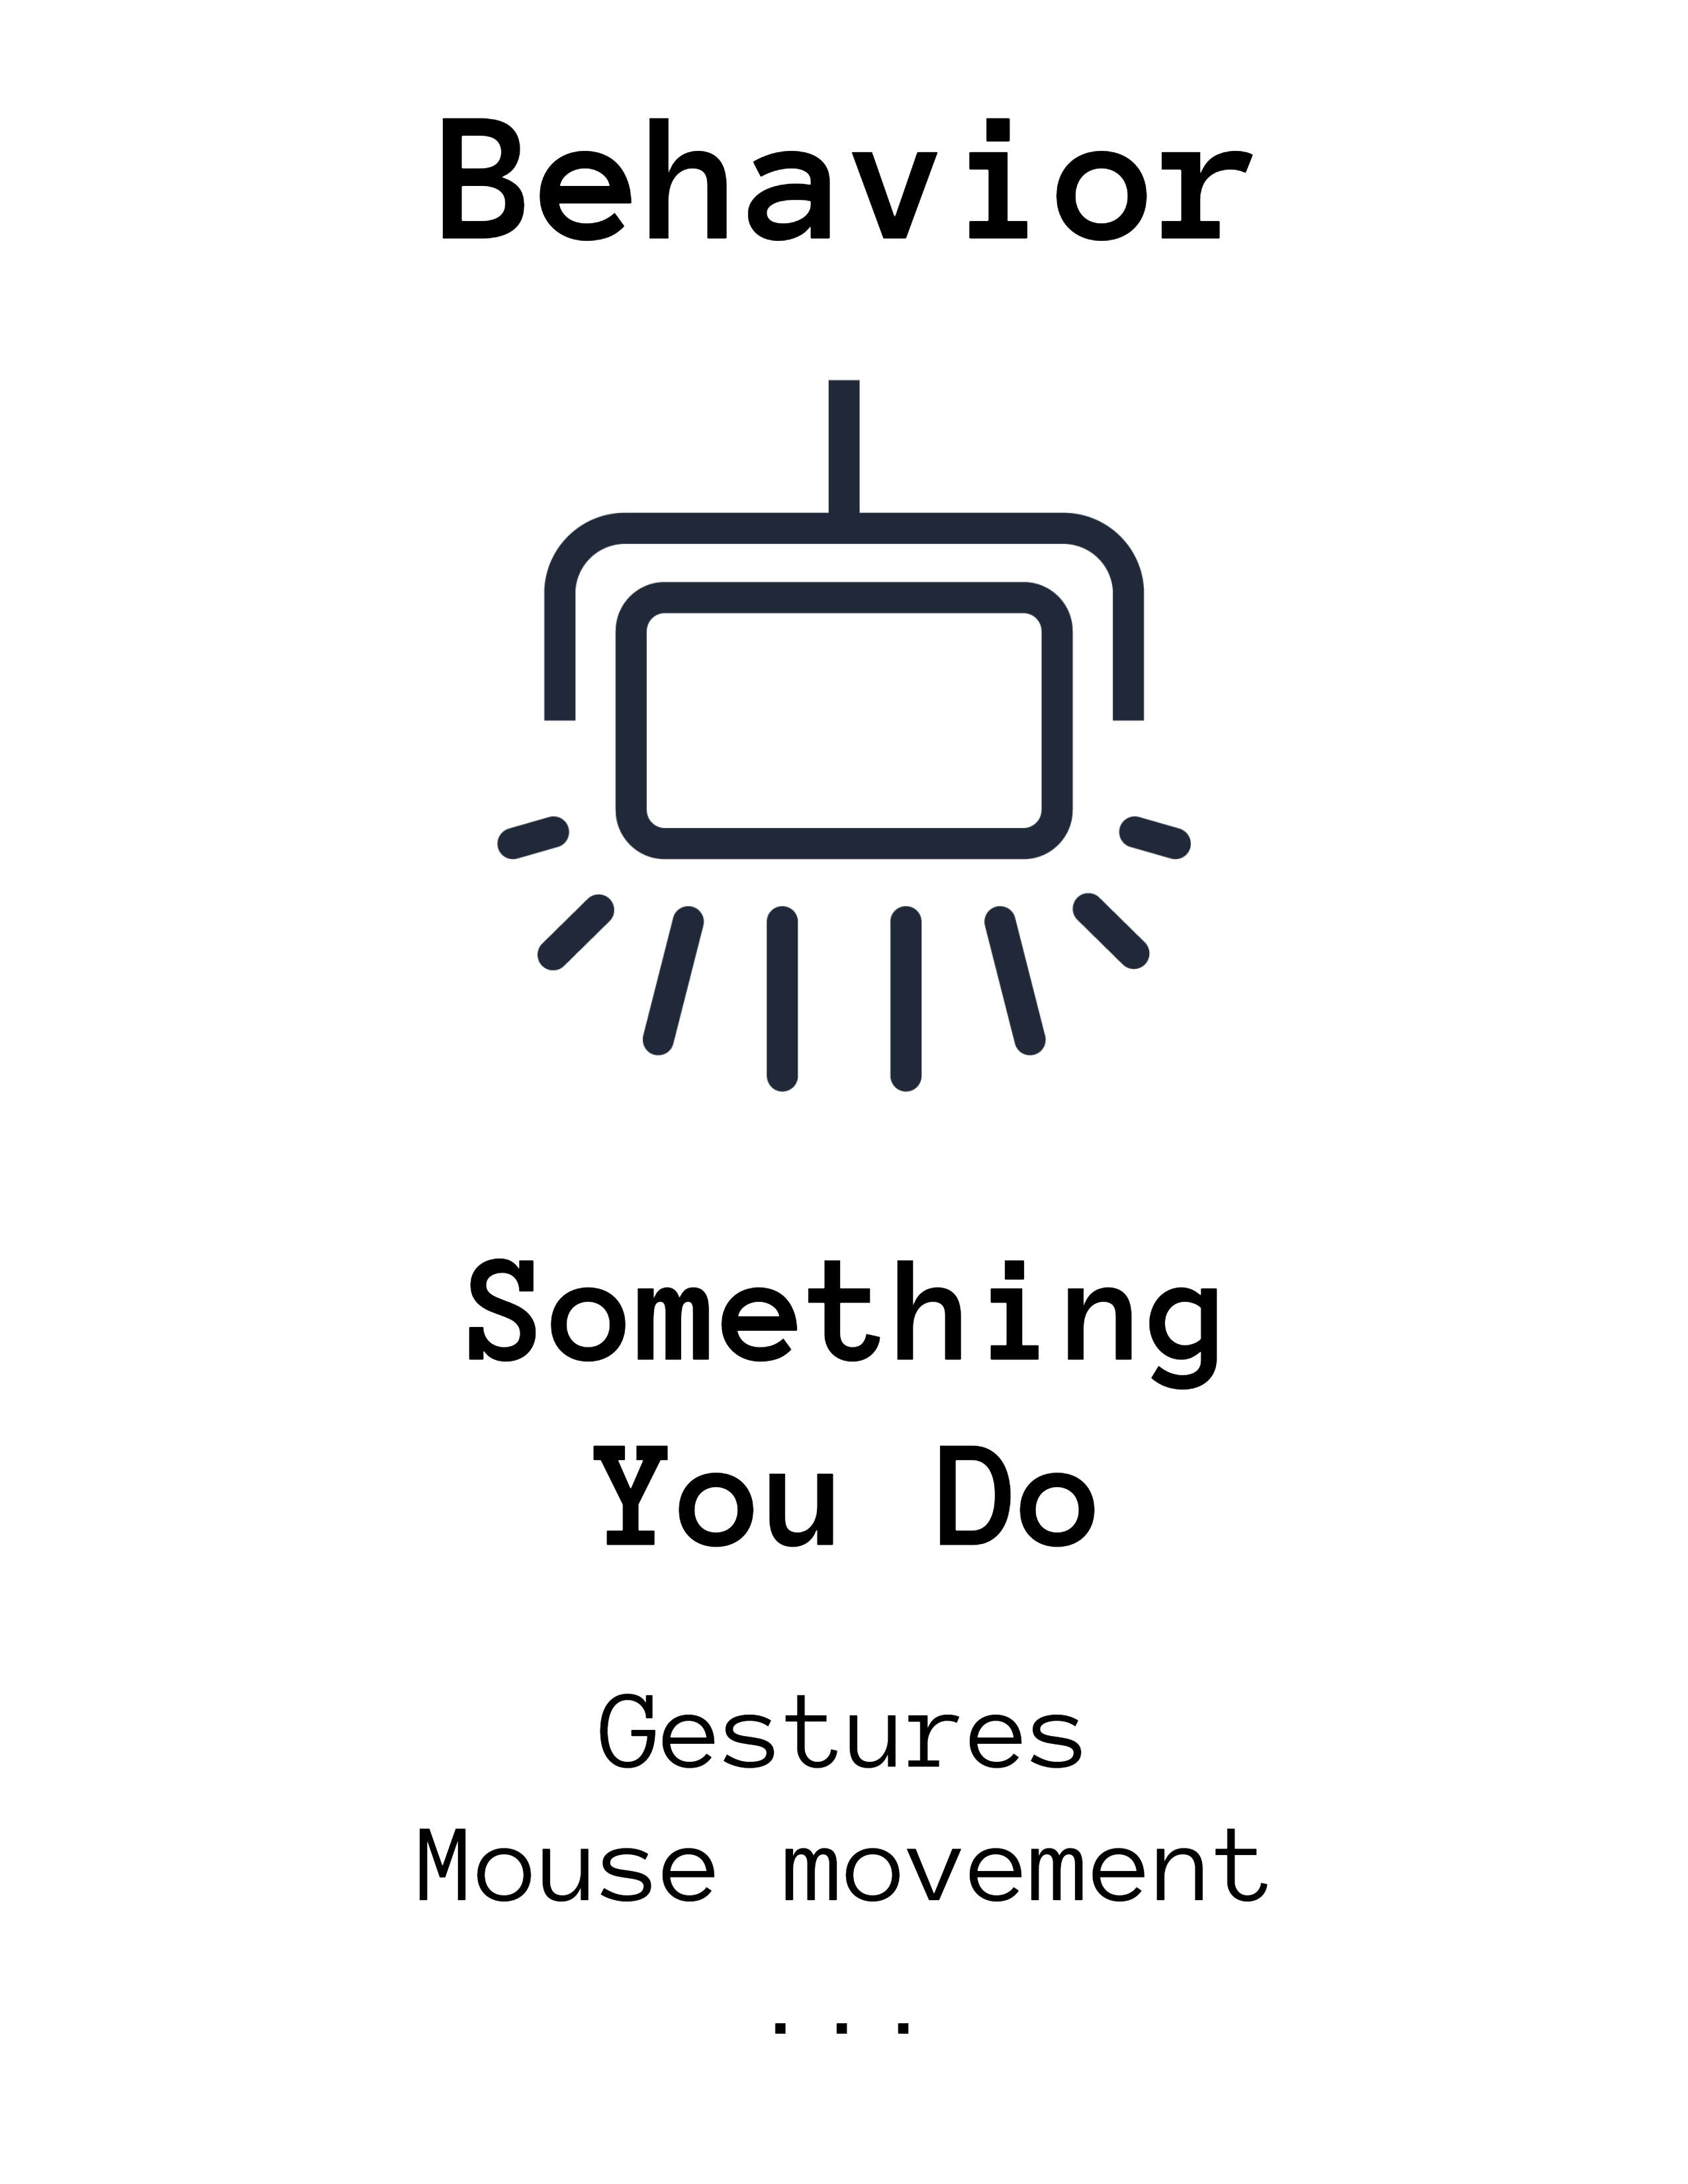
\includegraphics[width=0.6\textwidth]{img/behavior-final.png}
  \caption{Behavior factor}
  \label{fig:behavior-factor}
\end{figure}

% REF: https://www.sumologic.com/glossary/authentication-factor/
% https://www.globalknowledge.com/us-en/resources/resource-library/articles/the-three-types-of-multi-factor-authentication-mfa/
% https://www.aratek.co/news/5-authentication-factors-a-guide-from-passwords-to-biometrics

\newpage
\section{Risk Levels}

\chapter{Keycloak}
Keycloak

\section{Service Provider Interface}

\end{markdown*}


\shorthandon{-}

\chapter{Existing solutions}
\shorthandoff{-}
\begin{markdown*}{%
  hybrid,
  definitionLists,
  footnotes,
  inlineFootnotes,
  hashEnumerators,
  fencedCode,
  citations,
  citationNbsps,
  pipeTables,
  tableCaptions,
}

This specific part of the thesis is focused on the analysis of existing solutions provided by other vendors that are present on the market.
It is very beneficial to be aware of solutions for Adaptive Authentication as there are already some companies and institutions that are trying to solve the same problem as is touched on in this thesis.

The intention behind analyzing existing solutions is to get information from the other vendors in order not to reinvent the wheel.
In order to create an optimal solution for Adaptive authentication, it is advantageous to recognize common patterns in these solutions, aggregate the best parts, enhance them, and tailor them to the needs of Keycloak. 

In the following sections, there are some brief descriptions of products provided by the mentioned vendors.
The list of existing solutions and their ordering is not sorted by any particular keys but rather gathered as the most promising and exciting solutions.

\section{Okta}
Okta is an identity management company that provides cloud-based solutions for businesses to connect people and technology securely.
Okta offers a platform that enables organizations to manage and secure user authentication, access control, and identity governance across various applications and devices.
The company's services include single sign-on, multi-factor authentication, lifecycle management, and API access management.
Okta describes its Adaptive and risk-based capabilities as follows:

"User and risk levels are always changing; your security should be able to keep up.
Okta Adaptive MFA allows for dynamic policy changes and step-up authentication in response to changes in user and device behavior, location, or other contexts.
Adaptive MFA supports detection and authentication challenges for riskier situations like":

SOURCE: https://www.okta.com/sites/default/files/okta_mfa-datasheet.pdf

\begin{itemize}
    \item Use of weak/breached passwords
    \item Proxy use
    \item Geographic location and zone changes
    \item Brute force and denial-of-service attacks
    \item Use of new/untrusted devices
    \item Indications of anomalous behavior
\end{itemize}

\section{Something}
Something

\section{Common patterns}

\end{markdown*}

\chapter{Analysis}
\shorthandoff{-}
\shorthandoff{-}
\begin{markdown*}{%
  hybrid,
  definitionLists,
  footnotes,
  inlineFootnotes,
  hashEnumerators,
  fencedCode,
  citations,
  citationNbsps,
  pipeTables,
  tableCaptions,
}

\section{Necessary parts}
TODO -


\end{markdown*}
\shorthandon{-}


\chapter{Implementation}
\shorthandoff{-}
\begin{markdown*}{%
  hybrid,
  definitionLists,
  footnotes,
  inlineFootnotes,
  hashEnumerators,
  fencedCode,
  citations,
  citationNbsps,
  pipeTables,
  tableCaptions,
}

IMPLEMENTATION
\end{markdown*}
\shorthandon{-}

\chapter{Inserting the bibliography}
After linking a bibliography data\-base files to the document using
the \verb"\"\texttt{thesis\discretionary{-}{}{}setup\{bib\discretionary{=}{=}{=}%
\{\textit{file1},\textit{file2},\,\ldots\,\}\}} command, you can
start citing the entries. This is just dummy text
\parencite{borgman03} lightly sprinkled with citations
\parencite[p.~123]{greenberg98}. Several sources can be cited at
once: \cite{borgman03,greenberg98,thanh01}.
\citetitle{greenberg98} was written by \citeauthor{greenberg98} in
\citeyear{greenberg98}. We can also produce \textcite{greenberg98}%
\ or %% Let us define a compound command:
\def\citeauthoryear#1{(\textcite{#1},~\citeyear{#1})}%
\citeauthoryear{greenberg98}%
. The full bibliographic citation is:
\emph{\fullcite{greenberg98}}. We can easily insert a bibliographic
citation into the footnote\footfullcite{greenberg98}.

The \verb"\nocite" command will not generate any
output\nocite{muni}, but it will insert its arguments into
the bibliography. The \verb"\nocite{*}" command will insert all the
records in the bibliography database file into the bibliography.
Try uncommenting the command
%% \nocite{*}
and watch the bibliography section come apart at the seams.

When typesetting the document for the first time, citing a
\texttt{work} will expand to [\textbf{work}] and the
\verb"\printbibliography" command will produce no output. It is now
necessary to generate the bibliography by running \texttt{biber
\jobname.bcf} from the command line and then by typesetting the
document again twice. During the first run, the bibliography
section and the citations will be typeset, and in the second run,
the bibliography section will appear in the table of contents.

The \texttt{biber} command needs to be executed from within the
directory, where the \LaTeX\ source file is located. In Windows,
the command line can be opened in a directory by holding down the
\textsf{Shift} key and by clicking the right mouse button while
hovering the cursor over a directory.  Select the \textsf{Open
Command Window Here} option in the context menu that opens shortly
afterwards.

With online services -- such as Overleaf -- or when using an
automatic tool -- such as \LaTeX MK -- all commands are executed
automatically. When you omit the \verb"\printbibliography" command,
its location will be decided by the template.

  \printbibliography[heading=bibintoc] %% Print the bibliography.


\appendix %% Start the appendices.
\chapter{An appendix}
Here you can insert the appendices of your thesis.

\end{document}
